\documentclass[10pt,twocolumn]{article}

\usepackage[a4paper,margin=18mm,columnsep=8mm]{geometry}
\usepackage[T1]{fontenc}
\usepackage[utf8]{inputenc}
\usepackage{lmodern}
\usepackage{microtype}
\usepackage{amsmath,amssymb}
\usepackage{graphicx}
\usepackage{booktabs}
\usepackage{siunitx}
\sisetup{per-mode=fraction, inter-unit-product =\ensuremath{{}\cdot{}}}
\usepackage{balance}
\usepackage{tikz}
\usetikzlibrary{decorations.pathmorphing}
\usetikzlibrary{arrows.meta}
\usepackage{hyperref}
\usepackage[backend=biber,style=numeric,sorting=none,maxnames=6,url=false,doi=true,isbn=false,giveninits=true]{biblatex}
\addbibresource{lio.bib}
\AtBeginBibliography{\footnotesize}

\definecolor{Espresso}{HTML}{3B2F2F}
\definecolor{Cream}{HTML}{FFF7EA}
\definecolor{Sand}{HTML}{F1D6B8}
\definecolor{Terracotta}{HTML}{C96F4A}
\definecolor{Olive}{HTML}{7D8B52}
\definecolor{Plum}{HTML}{6F4E7C}

\newcommand{\keywords}[1]{\par\medskip\noindent\textbf{Keywords:} #1}

\title{Sensitivity Comparison of Atomic Interferometry and Deflectometry for Gravitational Measurements on Positronium Using Monte Carlo Simulations}

\author{
Mateusz Winiarski$^{1}$, Sebastiano Mariazzi$^{2,3}$, Roberto S. Brusa$^{2,3}$,\\
Paweł Moskal$^{1,4}$, and Sushil Sharma$^{1,4}$\\[1ex]
\small $^{1}$Faculty of Physics, Astronomy and Applied Computer Science, Jagiellonian University, Kraków, Poland\\
\small $^{2}$Department of Physics, University of Trento, Povo, Trento, Italy\\
\small $^{3}$TIFPA/INFN Trento, Povo, Trento, Italy\\
\small $^{4}$Center for Theranostics, Jagiellonian University, Kraków, Poland
}

\date{}

\begin{document}

\maketitle

\begin{abstract}
Positronium, a bound state of an electron and a positron, provides a clean system for testing fundamental interactions involving antimatter. We investigate the feasibility of measuring gravitational effects on metastable positronium using atom-interferometric methods. Two concepts are compared: a classical moir\'e deflectometer based on physical gratings and a Mach--Zehnder matter-wave interferometer based on standing light waves. Monte Carlo simulations account for the velocity, angular divergence, lifetime, trajectories, and decay positions of individual positronium atoms. The results indicate a minimum detectable acceleration of approximately $347.4\,g_\oplus$ for the moir\'e configuration and $14.3\,g_\oplus$ for the Mach--Zehnder configuration for $8\cdot10^4$ simulated particle shots under the studied assumptions. The greater sensitivity of the Mach-Zehnder interferometer results primarily from the smaller grating period achievable with optical gratings and from the high transparency of the standing light waves, which avoids annihilation losses on the grating material.
\keywords{positronium, antimatter gravity, atomic interferometry, moir\'e deflectometer, Mach--Zehnder interferometer, Monte Carlo simulation}
\end{abstract}

\section{Introduction}

Testing the response of antimatter to gravity is an important experimental challenge. Positronium (Ps), an electrically neutral bound state of an electron and a positron (Fig.~\ref{fig:positronium}), offers a particularly clean system for investigating fundamental interactions involving antimatter\cite{Bass_Mariazzi_Moskal_Stepien_2023}. Its neutrality reduces the influence of stray electric fields compared with charged antiparticles, while its simple leptonic structure enables precise theoretical predictions.

The principal difficulty is the short positronium lifetime. The ground-state ortho-positronium lifetime is approximately $142\,\mathrm{ns}$, whereas para-positronium decays after approximately $125\,\mathrm{ps}$. The metastable $2^3S$ state has a substantially longer lifetime of $1.142\,\si{\micro\second}$ and is therefore the most promising candidate for gravity measurements\cite{Mariazzi_Caravita_Doser_Nebbia_Brusa_2020}. A positron-to-positronium converter followed by ultraviolet excitation and Doppler selection may produce approximately $1.3\cdot10^5$ metastable Ps atoms with characteristic velocities near $10^5\,\si{\meter\per\second}$. A collimation slit can then form the beam required for an interferometric measurement.

This work compares two instruments: a classical moir\'e deflectometer and a quantum Mach--Zehnder interferometer. We use Monte Carlo simulations to evaluate their response to a uniform acceleration and to estimate the smallest detectable acceleration for experimentally relevant beam parameters.

\begin{figure}[ht!]
  \centering
  \resizebox{0.5\linewidth}{!}{\definecolor{Espresso}{HTML}{3B2F2F}
\definecolor{Cream}{HTML}{FFF7EA}
\definecolor{Sand}{HTML}{F1D6B8}
\definecolor{Terracotta}{HTML}{C96F4A}
\definecolor{Olive}{HTML}{7D8B52}
\definecolor{Plum}{HTML}{6F4E7C}
\definecolor{organiserblue}{HTML}{2E6F9E}

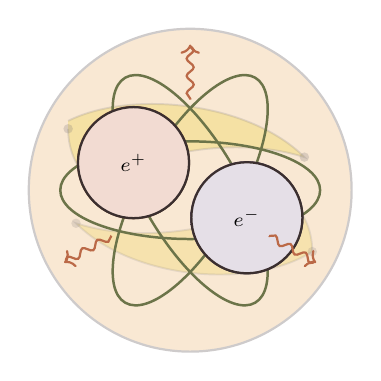
\begin{tikzpicture}[
  x=1cm,y=1cm,
  particle/.style={circle,draw=Espresso,line width=0.8pt,minimum size=1.41cm,inner sep=0pt,font=\scriptsize\bfseries},
  orbit/.style={draw=Olive!75!Espresso,line width=0.9pt},
  photon/.style={decorate,decoration={snake,amplitude=0.45mm,segment length=2.2mm},line width=0.8pt,Terracotta!90!Espresso}
]
  \fill[Sand!45!Cream] (0,0) circle (2.05);
  \draw[Espresso!25,line width=0.8pt] (0,0) circle (2.05);

  \begin{scope}[opacity=0.25]
    \fill[Terracotta!35!yellow]
      (-1.55,0.88)
      .. controls (-0.75,1.28) and (0.75,1.12) .. (1.45,0.42)
      .. controls (0.62,0.68) and (-0.42,0.52) .. (-1.20,0.08)
      .. controls (-1.42,0.22) and (-1.55,0.48) .. (-1.55,0.78)
      -- cycle;
    \draw[Espresso!55,line width=0.7pt]
      (-1.55,0.88)
      .. controls (-0.75,1.28) and (0.75,1.12) .. (1.45,0.42)
      .. controls (0.62,0.68) and (-0.42,0.52) .. (-1.20,0.08)
      .. controls (-1.42,0.22) and (-1.55,0.48) .. (-1.55,0.78);
    \fill[Espresso!65] (-1.55,0.78) circle (0.06);
    \fill[Espresso!65] (1.45,0.42) circle (0.06);
  \end{scope}

  \begin{scope}[opacity=0.2,rotate=180]
    \fill[Terracotta!35!yellow]
      (-1.55,0.78)
      .. controls (-0.75,1.28) and (0.75,1.12) .. (1.45,0.42)
      .. controls (0.62,0.68) and (-0.42,0.52) .. (-1.20,0.08)
      .. controls (-1.42,0.22) and (-1.55,0.48) .. (-1.55,0.78)
      -- cycle;
    \draw[Espresso!55,line width=0.7pt]
      (-1.55,0.78)
      .. controls (-0.75,1.28) and (0.75,1.12) .. (1.45,0.42)
      .. controls (0.62,0.68) and (-0.42,0.52) .. (-1.20,0.08)
      .. controls (-1.42,0.22) and (-1.55,0.48) .. (-1.55,0.78);
    \fill[Espresso!65] (-1.55,0.78) circle (0.06);
    \fill[Espresso!65] (1.45,0.42) circle (0.06);
  \end{scope}

  \draw[orbit,rotate=0] (0,0) ellipse (1.65 and 0.62);
  \draw[orbit,rotate=60] (0,0) ellipse (1.65 and 0.62);
  \draw[orbit,rotate=-60] (0,0) ellipse (1.65 and 0.62);

  \shade[ball color=Terracotta!85!white] (-0.72,0.35) circle (0.72);
  \node[particle,fill=Terracotta!25] at (-0.72,0.35) {$e^+$};

  \shade[ball color=Plum!75!white] (0.72,-0.35) circle (0.72);
  \node[particle,fill=Plum!18] at (0.72,-0.35) {$e^-$};

  % \node[font=\scriptsize\bfseries,Espresso] at (0,-2.45) {positronium};
  % \node[font=\scriptsize,Espresso,align=center] at (0,-2.85) {bound state of\\electron and positron};

  % Three emitted photons at 120 degrees: net momentum is zero.
  \draw[photon,<-] (0,1.85) -- (0,1.15);
  \draw[photon,<-] (-1.60,-0.92) -- (-1.00,-0.58);
  \draw[photon,<-] (1.60,-0.92) -- (1.00,-0.58);
\end{tikzpicture}}
  \caption{Schematic representation of positronium as an electron--positron bound state. The metastable $2^3S$ state provides a longer observation time than the ground states.}
  \label{fig:positronium}
\end{figure}

\section{Interferometer concepts}

\subsection{Moir\'e deflectometer}

A moir\'e deflectometer (Fig.~\ref{fig:moire-principle}) is a classical device consisting of two identical physical gratings with period $d$ in the micrometer range. The gratings transmit particles only within selected spatial intervals. When illuminated by a beam with finite angular divergence, they generate a periodic moir\'e pattern with the same period $d$. An external force changes the particle trajectories and shifts the detected pattern.

For two equal propagation distances $L$, the gravitational deflection increases with the time of flight. The useful signal is the displacement of the periodic transmission pattern relative to the zero-acceleration case. The method does not require coherent matter waves, which simplifies its interpretation and makes it suitable for implementation in particle-transport simulation frameworks such as Geant4.

\begin{figure}[ht!]
  \centering
  \resizebox{\linewidth}{!}{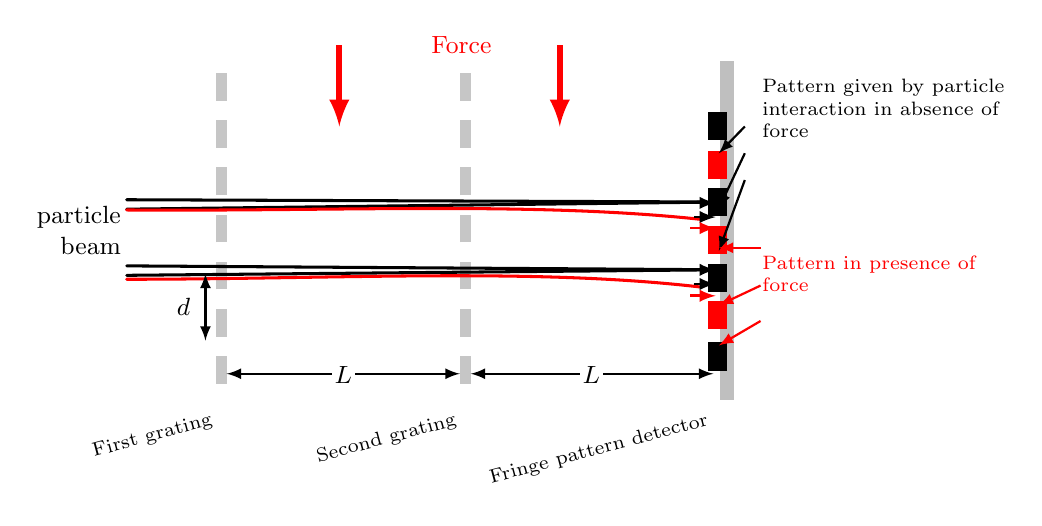
\begin{tikzpicture}[
  x=1cm,y=1cm,
  beam/.style={line width=1.1pt,line cap=round},
  force/.style={-latex,red,line width=2.3pt},
  label/.style={font=\small},
  smalllabel/.style={font=\scriptsize},
  dim/.style={latex-latex,line width=0.8pt},
  callout/.style={-latex,line width=0.8pt},
  redcallout/.style={-latex,red,line width=0.8pt}
]
  \def\gOne{1.25}
  \def\gTwo{4.35}
  \def\det{7.55}

  \foreach \x in {\gOne,\gTwo}{
    \foreach \y in {0.45,1.05,1.65,2.25,2.85,3.45,4.05}{
      \draw[gray!45,line width=4pt] (\x,\y) -- (\x,\y+0.35);
    }
  }

  \draw[gray!50,line width=5pt] (\det+0.12,0.25) -- (\det+0.12,4.55);
  \foreach \y/\c in {0.62/black,1.15/red,1.62/black,2.10/red,2.58/black,3.05/red,3.55/black}{
    \draw[\c,line width=7pt] (\det,\y) -- (\det,\y+0.36);
  }

  \node[label,align=right,anchor=east] at (0.10,2.40) {particle\\beam};
  \node[label,red] at (4.30,4.75) {Force};
  \draw[force] (2.75,4.75) -- (2.75,3.72);
  \draw[force] (5.55,4.75) -- (5.55,3.72);

  \foreach \dy in {-0.05,0.07}{
    \draw[beam,black] (0.05,2.72+\dy) -- (\det-0.20,2.76+0.03*\dy);
    \draw[beam,black] (0.05,1.88+\dy) -- (\det-0.20,1.90+0.03*\dy);
  }
  \draw[beam,red] (0.05,2.66) .. controls (2.7,2.64) and (5.2,2.77) .. (\det-0.20,2.54);
  \draw[beam,red] (0.05,1.78) .. controls (2.7,1.78) and (5.2,1.93) .. (\det-0.20,1.68);

  \foreach \y in {2.57,2.75,1.72,1.90}{
    \draw[-latex,line width=1pt] (\det-0.30,\y) -- (\det-0.02,\y);
  }
  \draw[-latex,red,line width=1pt] (\det-0.34,2.43) -- (\det-0.02,2.43);
  \draw[-latex,red,line width=1pt] (\det-0.34,1.57) -- (\det-0.02,1.57);

  \draw[dim] (\gOne-0.20,1.00) -- (\gOne-0.20,1.85);
  \node[label,fill=white,inner sep=1pt] at (\gOne-0.48,1.43) {$d$};

  \draw[dim] (\gOne+0.07,0.58) -- (\gTwo-0.07,0.58);
  \node[label,fill=white,inner sep=1pt] at ({(\gOne+\gTwo)/2},0.56) {$L$};
  \draw[dim] (\gTwo+0.07,0.58) -- (\det-0.05,0.58);
  \node[label,fill=white,inner sep=1pt] at ({(\gTwo+\det)/2},0.56) {$L$};

  \node[smalllabel,align=center,rotate=15,anchor=east] at (\gOne,0.02) {First grating};
  \node[smalllabel,align=center,rotate=15,anchor=east] at (\gTwo,0.02) {Second grating};
  \node[smalllabel,align=center,rotate=15,anchor=east] at (\det,0.02) {Fringe pattern detector};

  \node[smalllabel,align=left,anchor=west] (absent) at (8.00,3.95) {Pattern given by particle\\interaction in absence of\\force};
  \draw[callout] (7.90,3.72) -- (\det+0.02,3.38);
  \draw[callout] (7.90,3.38) -- (\det+0.02,2.68);
  \draw[callout] (7.90,3.04) -- (\det+0.02,2.14);

  \node[smalllabel,align=left,anchor=west,red] at (8.00,1.85) {Pattern in presence of\\force};
  \draw[redcallout] (8.10,2.18) -- (\det+0.02,2.18);
  \draw[redcallout] (8.10,1.70) -- (\det+0.02,1.45);
  \draw[redcallout] (8.10,1.25) -- (\det+0.02,0.94);
\end{tikzpicture}}
  \caption{Operating principle of the moir\'e deflectometer. A force changes the particle trajectories and shifts the fringe pattern generated by two physical gratings. Adapted from Refs.~\cite{Mariazzi_Caravita_Doser_Nebbia_Brusa_2020,Oberthaler_Bernet_Rasel_Schmiedmayer_Zeilinger_1996}.}
  \label{fig:moire-principle}
\end{figure}

\subsection{Mach--Zehnder interferometer}

The Mach--Zehnder configuration (Fig.~\ref{fig:mz-principle}) operates in the de Broglie matter-wave regime\cite{Oberthaler_Bernet_Rasel_Schmiedmayer_Zeilinger_1996,Oberthaler_2002}. The first grating acts as a beam splitter and the second as a recombiner. An external force changes both the particle trajectories and their phases, thereby shifting the interference fringes. Standing laser waves can serve as optical gratings, reducing the grating period to the hundred-nanometer range. This substantially increases sensitivity to small phase and pattern shifts. In addition to the smaller period, standing light waves are almost fully transparent to the positronium beam, so atoms are not lost by annihilation on the grating, unlike in the moiré configuration.

The interferometer requires sufficient transverse coherence. A beam with excessive angular divergence averages over different phases and reduces the fringe contrast. Consequently, the beam divergence must be optimized by balancing the transmitted particle number against the visibility of the interference pattern.

\begin{figure}[ht!]
  \centering
  \resizebox{\linewidth}{!}{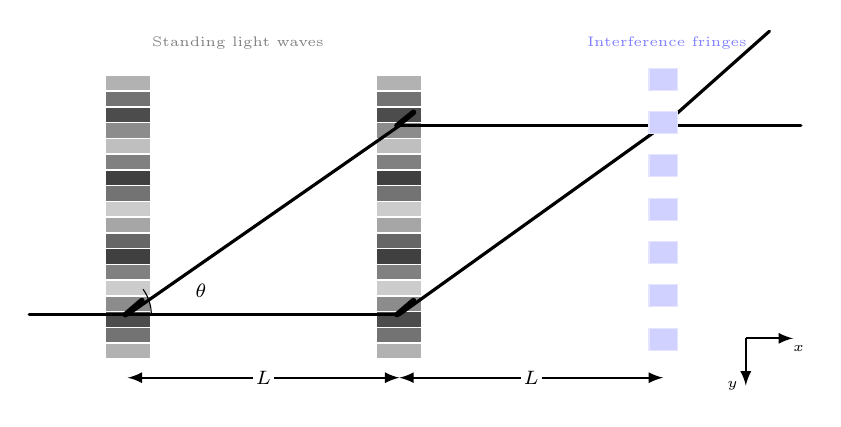
\begin{tikzpicture}[
  x=1cm,y=1cm,
  ray/.style={line width=1.15pt,line cap=round},
  dim/.style={latex-latex,line width=0.8pt},
  label/.style={font=\scriptsize},
  smalllabel/.style={font=\tiny},
  fringe/.style={fill=blue!18,draw=blue!10}
]
  \def\gA{1.30}
  \def\gB{4.75}
  \def\scr{8.10}

  % \node[smalllabel,font=\scriptsize\bfseries] at (4.60,5.85) {Mach--Zehnder interferometer};
  \node[smalllabel,black!50] at (2.70,4.90) {Standing light waves};
  \node[smalllabel,blue!50] at (8.15,4.90) {Interference fringes};

  \foreach \x in {\gA,\gB}{
    \foreach \y/\shade in {0.90/30,1.10/55,1.30/70,1.50/45,1.70/20,1.90/50,2.10/75,2.30/60,2.50/35,2.70/20,2.90/55,3.10/75,3.30/50,3.50/25,3.70/45,3.90/70,4.10/55,4.30/30}{
      \fill[black!\shade] (\x-0.28,\y) rectangle (\x+0.28,\y+0.18);
    }
  }

  \draw[ray] (0.05,1.45) -- (\gA,1.45);
  \draw[ray] (\gA,1.45) -- (\gB,3.85);
  \draw[ray] (\gB,3.85) -- (\scr,3.85);
  \draw[ray] (\gA,1.45) -- (\gB,1.45);
  \draw[ray] (\gB,1.45) -- (\scr,3.85);
  \draw[ray] (\scr,3.85) -- (9.85,3.85);
  \draw[ray] (\scr,3.85) -- (9.45,5.05);

  \draw[ray,line width=2pt] (\gA-0.03,1.45) -- (\gA+0.18,1.63);
  \draw[ray,line width=2pt] (\gB-0.03,1.45) -- (\gB+0.18,1.63);
  \draw[ray,line width=2pt] (\gB-0.03,3.85) -- (\gB+0.18,4.02);

  \draw[thin] (\gA+0.30,1.45) arc[start angle=0,end angle=36,radius=0.55];
  \node[label] at (\gA+0.93,1.76) {$\theta$};

  \foreach \y in {1.00,1.55,2.10,2.65,3.20,3.75,4.30}{
    \path[fringe] (\scr-0.18,\y) rectangle (\scr+0.18,\y+0.28);
  }

  \draw[dim] (\gA,0.65) -- (\gB,0.65);
  \node[label,fill=white,inner sep=1pt] at ({(\gA+\gB)/2},0.65) {$L$};
  \draw[dim] (\gB,0.65) -- (\scr,0.65);
  \node[label,fill=white,inner sep=1pt] at ({(\gB+\scr)/2},0.65) {$L$};

  \draw[-latex,line width=0.8pt] (9.15,1.15) -- (9.75,1.15);
  \draw[-latex,line width=0.8pt] (9.15,1.15) -- (9.15,0.55);
  \node[smalllabel] at (9.82,1.02) {$x$};
  \node[smalllabel] at (8.98,0.55) {$y$};
\end{tikzpicture}}
  \caption{Schematic Mach--Zehnder matter-wave interferometer with standing-light-wave gratings and an interference-fringe detector. Adapted from Ref. \cite{Mariazzi_Caravita_Doser_Nebbia_Brusa_2020}.}
  \label{fig:mz-principle}
\end{figure}

\section{Pattern detection}

The microscopic fringe patterns cannot be measured directly with positronium decay detectors such as J-PET\cite{Kowalski_Wiślicki_Shopa_Raczyński_Klimaszewski_Curcenau_Czerwiński_Dulski_Gajos_Gorgol_etal._2018,Sharma_Baran_Brusa_Caravita_Chug_Coussat_Curceanu_Czerwiński_Dadgar_Dulski_etal._2023,doi:10.1126/sciadv.abh4394}. Specifically, the J-PET detector has an axial position resolution of approximately 2.5~cm, whereas the spatial shift of the positronium beam induced by Earth's gravitational field during the particle's short lifetime is on the sub-nanometer scale. To overcome this limitation, we consider a scanning detection scheme based on an additional physical grating and a stopper placed a few centimeters downstream\cite{Mariazzi_Caravita_Doser_Nebbia_Brusa_2020} (Fig.~\ref{fig:detection-geometry}). This third grating is essential, as it effectively converts a spatial displacement too small to resolve directly with J-PET into a measurable modulation of the count rate of atoms reaching the stopper.

The third grating is translated step by step over one period. At each relative position $y_3$, a separate Monte Carlo simulation is performed and particles decaying on the third grating, on the stopper, or in the space between them are counted. The resulting count rate is periodic in $y_3$ (Fig.~\ref{fig:detection}). In the present simulations, one period is sampled at 200 positions.

\begin{figure}[ht!]
  \centering
  \resizebox{\linewidth}{!}{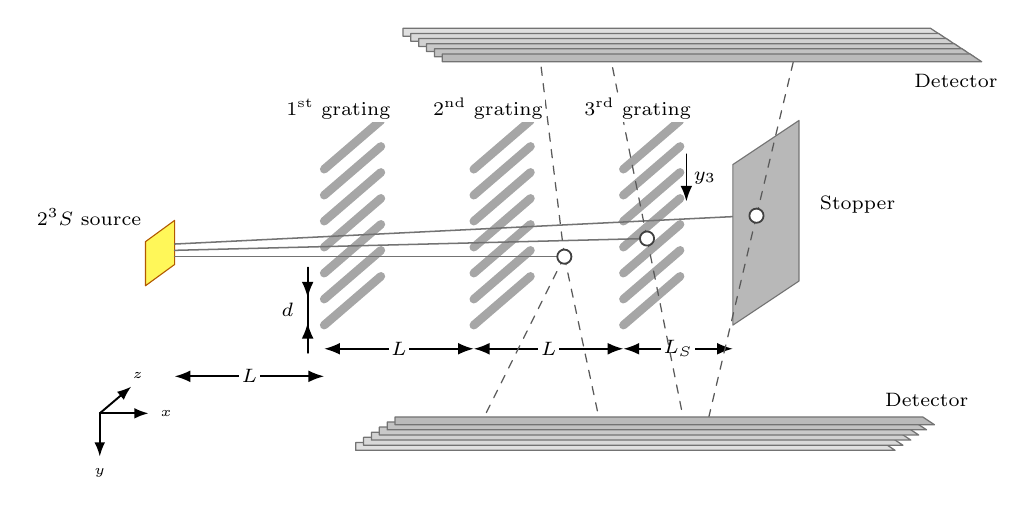
\begin{tikzpicture}[
  x=1cm,
  y=1cm,
  line cap=round,
  line join=round,
  label/.style={font=\scriptsize},
  smalllabel/.style={font=\tiny},
  beam/.style={draw=black!55,line width=0.55pt},
  photon/.style={draw=black!65,line width=0.45pt,dashed},
  dimension/.style={{Latex[length=2mm]}-{Latex[length=2mm]},line width=0.65pt},
  axis/.style={-{Latex[length=1.8mm]},line width=0.7pt}
]

  % Positronium source
  \fill[yellow!65] (-0.82,2.35) -- (-0.45,2.62) -- (-0.45,3.18)
      -- (-0.82,2.91) -- cycle;
  \draw[orange!70!black] (-0.82,2.35) -- (-0.45,2.62) -- (-0.45,3.18)
      -- (-0.82,2.91) -- cycle;
  \node[label,anchor=east] at (-0.75,3.22) {$2^3S$ source};

  % Three material gratings.  The repeated diagonal bars suggest depth.
  \foreach \gx/\name in {1.45/{1\textsuperscript{st} grating},
                          3.35/{2\textsuperscript{nd} grating},
                          5.25/{3\textsuperscript{rd} grating}} {
    \foreach \yy in {1.85,2.18,2.51,2.84,3.17,3.50,3.83} {
      \draw[black!35,line width=3.1pt]
        (\gx,\yy) -- ++(0.72,0.62);
    }
  }

  % Representative trajectories of the metastable positronium beam
  \draw[beam] (-0.45,2.72) -- (4.50,2.72);
  \draw[beam] (-0.45,2.80) -- (5.55,2.95);
  \draw[beam] (-0.45,2.88) -- (6.88,3.24);

  % Grating period d
  \draw[line width=0.65pt] (1.24,1.50) -- (1.24,2.58);
  \draw[-{Latex[length=2mm]},line width=0.65pt]
    (1.24,1.50) -- (1.24,1.88);
  \draw[-{Latex[length=2mm]},line width=0.65pt]
    (1.24,2.58) -- (1.24,2.20);
  \node[label,anchor=east] at (1.18,2.04) {$d$};

  % Equal distances between consecutive gratings
  \draw[dimension] (-0.45,1.20) -- (1.45,1.20);
  \node[label,fill=white,inner sep=1pt] at (0.50,1.20) {$L$};
  \draw[dimension] (1.45,1.55) -- (3.35,1.55);
  \node[label,fill=white,inner sep=1pt] at (2.40,1.55) {$L$};
  \draw[dimension] (3.35,1.55) -- (5.25,1.55);
  \node[label,fill=white,inner sep=1pt] at (4.30,1.55) {$L$};
  \draw[dimension] (5.25,1.55) -- (6.64,1.55);
  \node[label,fill=white,inner sep=1pt] at (5.945,1.55) {$L_S$};

  % Annihilation point and reconstructed vertical position
  % Highest beam at the stopper and middle beam at the third grating.
  \coordinate (decay) at (6.94,3.24);
  \coordinate (decaytwo) at (5.55,2.95);
  \coordinate (decaythree) at (4.50,2.72);
  \draw[-{Latex[length=2mm]},line width=0.65pt]
    (6.05,4.02) -- (6.05,3.42);
  \node[label,anchor=west] at (6.02,3.72) {$y_3$};

  % Stopper blocking the surviving positronium atoms
  \fill[black!28] (6.64,1.85) -- (7.48,2.41) -- (7.48,4.45)
      -- (6.64,3.89) -- cycle;
  \draw[black!55] (6.64,1.85) -- (7.48,2.41) -- (7.48,4.45)
      -- (6.64,3.89) -- cycle;
  \node[label,anchor=west] at (7.62,3.38) {Stopper};

  % Gamma rays from the annihilation point to opposite detector modules
  \draw[photon] (decay) -- (7.50,5.58);
  \draw[photon] (decay) -- (6.32,0.62);

  % A second reconstructed event, included as in the reference drawing
  \draw[photon] (decaytwo) -- (5.02,5.58);
  \draw[photon] (decaytwo) -- (6.02,0.62);

  % Three-photon annihilation from the third point
  \draw[photon] (decaythree) -- (4.15,5.58);
  \draw[photon] (decaythree) -- (3.45,0.62);
  \draw[photon] (decaythree) -- (4.95,0.62);

  % Annihilation points
  \draw[black!75,fill=white,line width=0.65pt] (decay) circle (0.09);
  \draw[black!75,fill=white,line width=0.65pt] (decaytwo) circle (0.09);
  \draw[black!75,fill=white,line width=0.65pt] (decaythree) circle (0.09);

  % Long scintillator modules above and below the apparatus
  \foreach \i in {0,...,5} {
    \pgfmathsetmacro{\dx}{0.10*\i}
    \pgfmathsetmacro{\dy}{0.065*\i}
    \pgfmathtruncatemacro{\detectorshade}{12+3*\i}
    \fill[black!\detectorshade]
      (2.45+\dx,5.62-\dy) -- (9.15+\dx,5.62-\dy)
      -- (9.30+\dx,5.52-\dy) -- (2.45+\dx,5.52-\dy) -- cycle;
    \draw[black!55,line width=0.45pt]
      (2.45+\dx,5.62-\dy) -- (9.15+\dx,5.62-\dy)
      -- (9.30+\dx,5.52-\dy) -- (2.45+\dx,5.52-\dy) -- cycle;
    \fill[black!\detectorshade]
      (1.85+\dx,0.36+\dy) -- (8.55+\dx,0.36+\dy)
      -- (8.70+\dx,0.26+\dy) -- (1.85+\dx,0.26+\dy) -- cycle;
    \draw[black!55,line width=0.45pt]
      (1.85+\dx,0.36+\dy) -- (8.55+\dx,0.36+\dy)
      -- (8.70+\dx,0.26+\dy) -- (1.85+\dx,0.26+\dy) -- cycle;
  }
  \node[label,anchor=west] at (8.82,4.95) {Detector};
  \node[label,anchor=west] at (8.45,0.90) {Detector};

  % Draw grating labels last so that the detector perspective does not hide them.
  \node[label,anchor=south,fill=white,inner sep=1pt] at (1.63,4.42)
    {1\textsuperscript{st} grating};
  \node[label,anchor=south,fill=white,inner sep=1pt] at (3.53,4.42)
    {2\textsuperscript{nd} grating};
  \node[label,anchor=south,fill=white,inner sep=1pt] at (5.43,4.42)
    {3\textsuperscript{rd} grating};

  % Coordinate system
  \coordinate (origin) at (-1.40,0.73);
  \draw[axis] (origin) -- ++(0.62,0);
  \draw[axis] (origin) -- ++(0,-0.55);
  \draw[axis] (origin) -- ++(0.40,0.34);
  \node[smalllabel,anchor=west] at (-0.75,0.73) {$x$};
  \node[smalllabel,anchor=north] at (-1.40,0.15) {$y$};
  \node[smalllabel,anchor=south east] at (-0.73,1.05) {$z$};

\end{tikzpicture}}
  \caption{Proposed scanning detection geometry. Adapted from Ref. \cite{Mariazzi_Caravita_Doser_Nebbia_Brusa_2020}.}
  \label{fig:detection-geometry}
\end{figure}

\begin{figure}[ht!]
  \centering
  \begin{minipage}[c]{\linewidth}
    \centering
    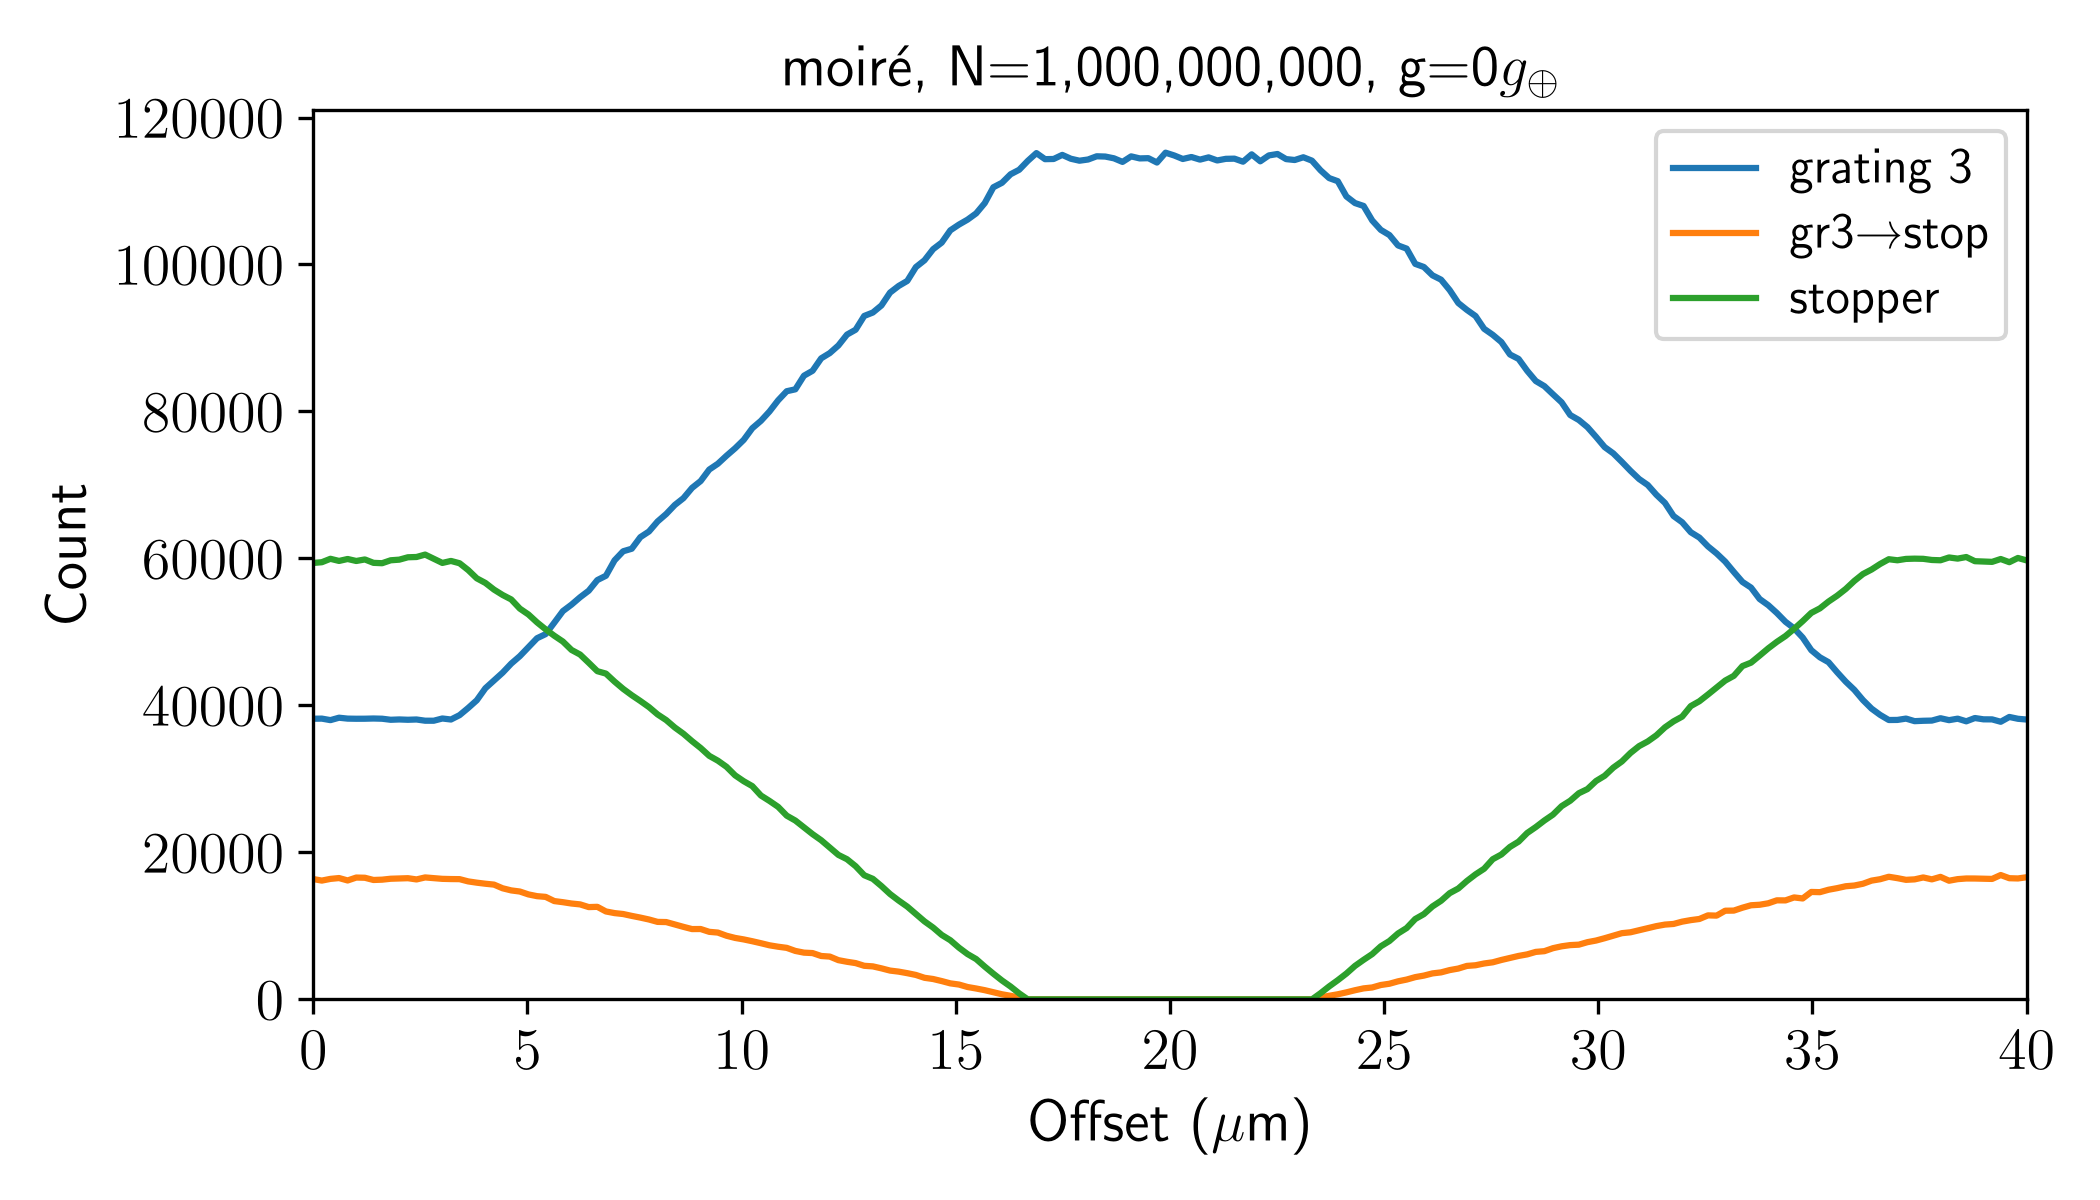
\includegraphics[width=\linewidth]{moire/moirepattern.png}
    \par\smallskip
    \footnotesize Simulated moir\'e transmission pattern.
  \end{minipage}\par\medskip
  \begin{minipage}[c]{\linewidth}
    \centering
    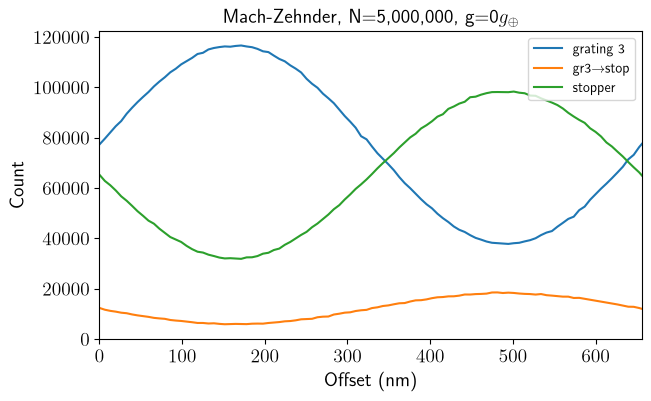
\includegraphics[width=\linewidth]{mach/mach_zehnder_pattern.png}
    \par\smallskip
    \footnotesize Simulated Mach--Zehnder transmission pattern.
  \end{minipage}
  \caption{Representative periodic signals obtained by scanning the third grating. The horizontal scales differ between the two interferometer concepts.}
  \label{fig:detection}
\end{figure}

\section{Monte Carlo model}

For both interferometer concepts, each simulated particle is assigned a velocity sampled from a Gaussian distribution, an incidence angle sampled from a uniform distribution, and a lifetime sampled from an exponential distribution.

For the moir\'e deflectometer, the particle trajectory under a uniform acceleration is calculated until it crosses a grating, reaches the stopper, or decays inside the apparatus. The simulated detection category is recorded for each position of the third grating.

For the Mach--Zehnder interferometer, particle survival through the apparatus is checked. The total phase includes the geometric contribution and the acceleration-induced phase shift for the sampled velocity. A quantum output path is then selected randomly according to the corresponding interference probability. The simulation records whether the particle exits through a bright or dark port and whether it crosses or is stopped by the third grating.

The sensitivity is quantified through the minimum detectable acceleration $a_{\min}$. The model incorporates its dependence on the grating period, fringe visibility, time of flight, and number of detected particles. The sensitivity is expected to scale approximately as
\begin{equation}
  a_{\min}\propto\frac{d}{C t^2\sqrt{N_{\mathrm{det}}}},
  \label{eq:acceleration-sensitivity}
\end{equation}
where $d$ is the grating period, $C$ is the fringe visibility (contrast), $t$ is the effective time of flight between the gratings (interrogation time), and $N_{\mathrm{det}}$ is the number of detected particles contributing to the pattern. For fixed geometry, contrast, and time of flight, this reduces to the statistical scaling $a_{\min}\propto1/\sqrt{N_{\mathrm{det}}}$.

\section{Results}

\subsection{Moir\'e deflectometer}

The simulated sensitivity depends strongly on the maximum beam-divergence angle $\theta_{\max}$ (Fig.~\ref{fig:moire-results}). Increasing the accepted divergence increases the number of particles in each shot, but a moir\'e deflectometer still requires a sufficiently collimated beam. For $8\cdot10^4$ particle shots, corresponding to approximately 5.3 weeks of continuous measurement under the assumed source conditions ((a bunch of $1.3\cdot10^5$ metastable Ps atoms produced every 40 s)), the studied configuration operating with a beam divergence of $17\,\mathrm{mrad}$ reaches $a_{\min} = (3408 \pm 31)\,\mathrm{m\,s^{-2}}$ (approximately $347.4\,g_\oplus$). Longer acquisition times may be estimated from the approximate $1/\sqrt{N_{\mathrm{det}}}$ scaling.

\begin{figure}[ht!]
  \centering
  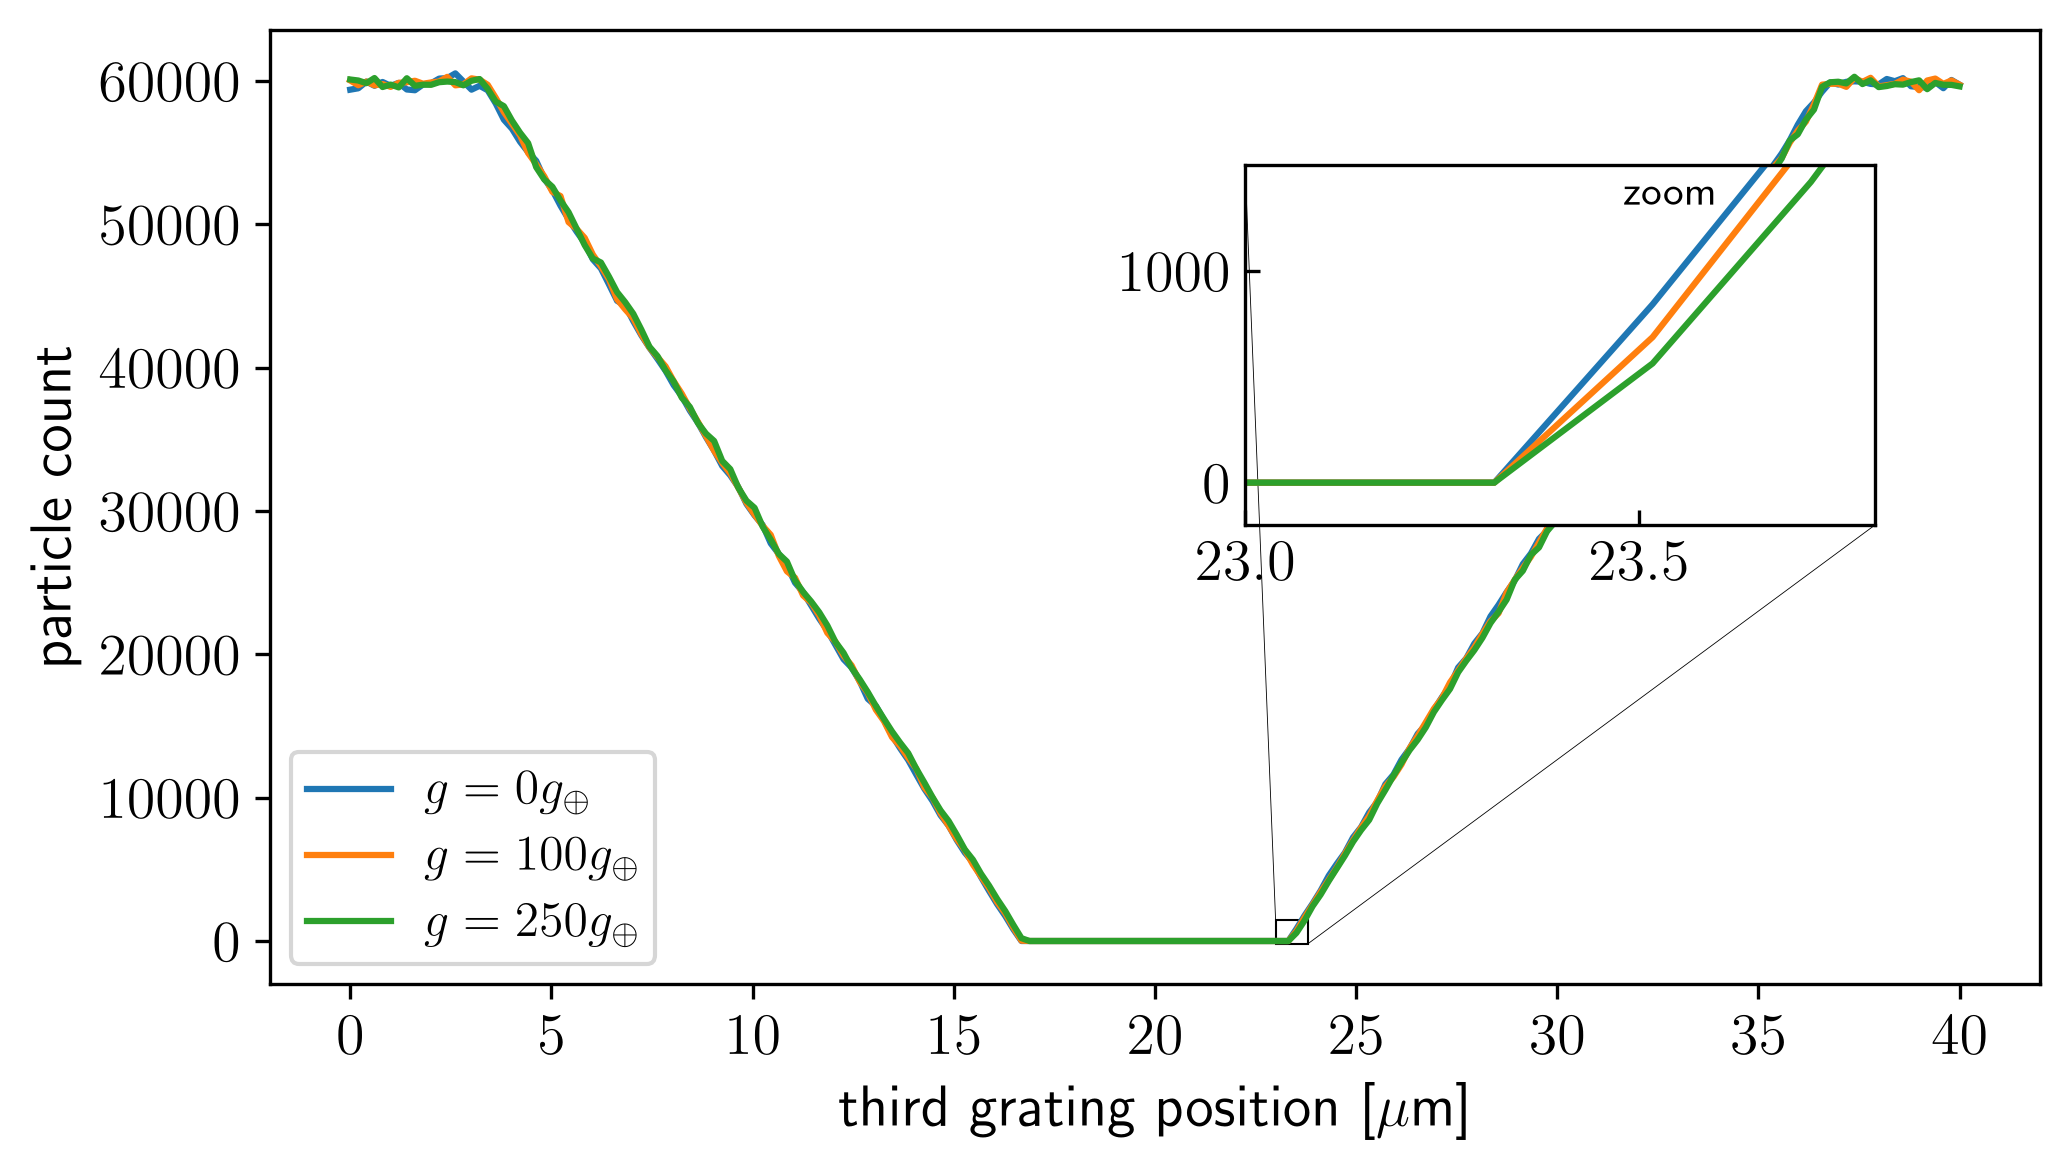
\includegraphics[width=\linewidth]{moire/moire-inset.png}\par\medskip
  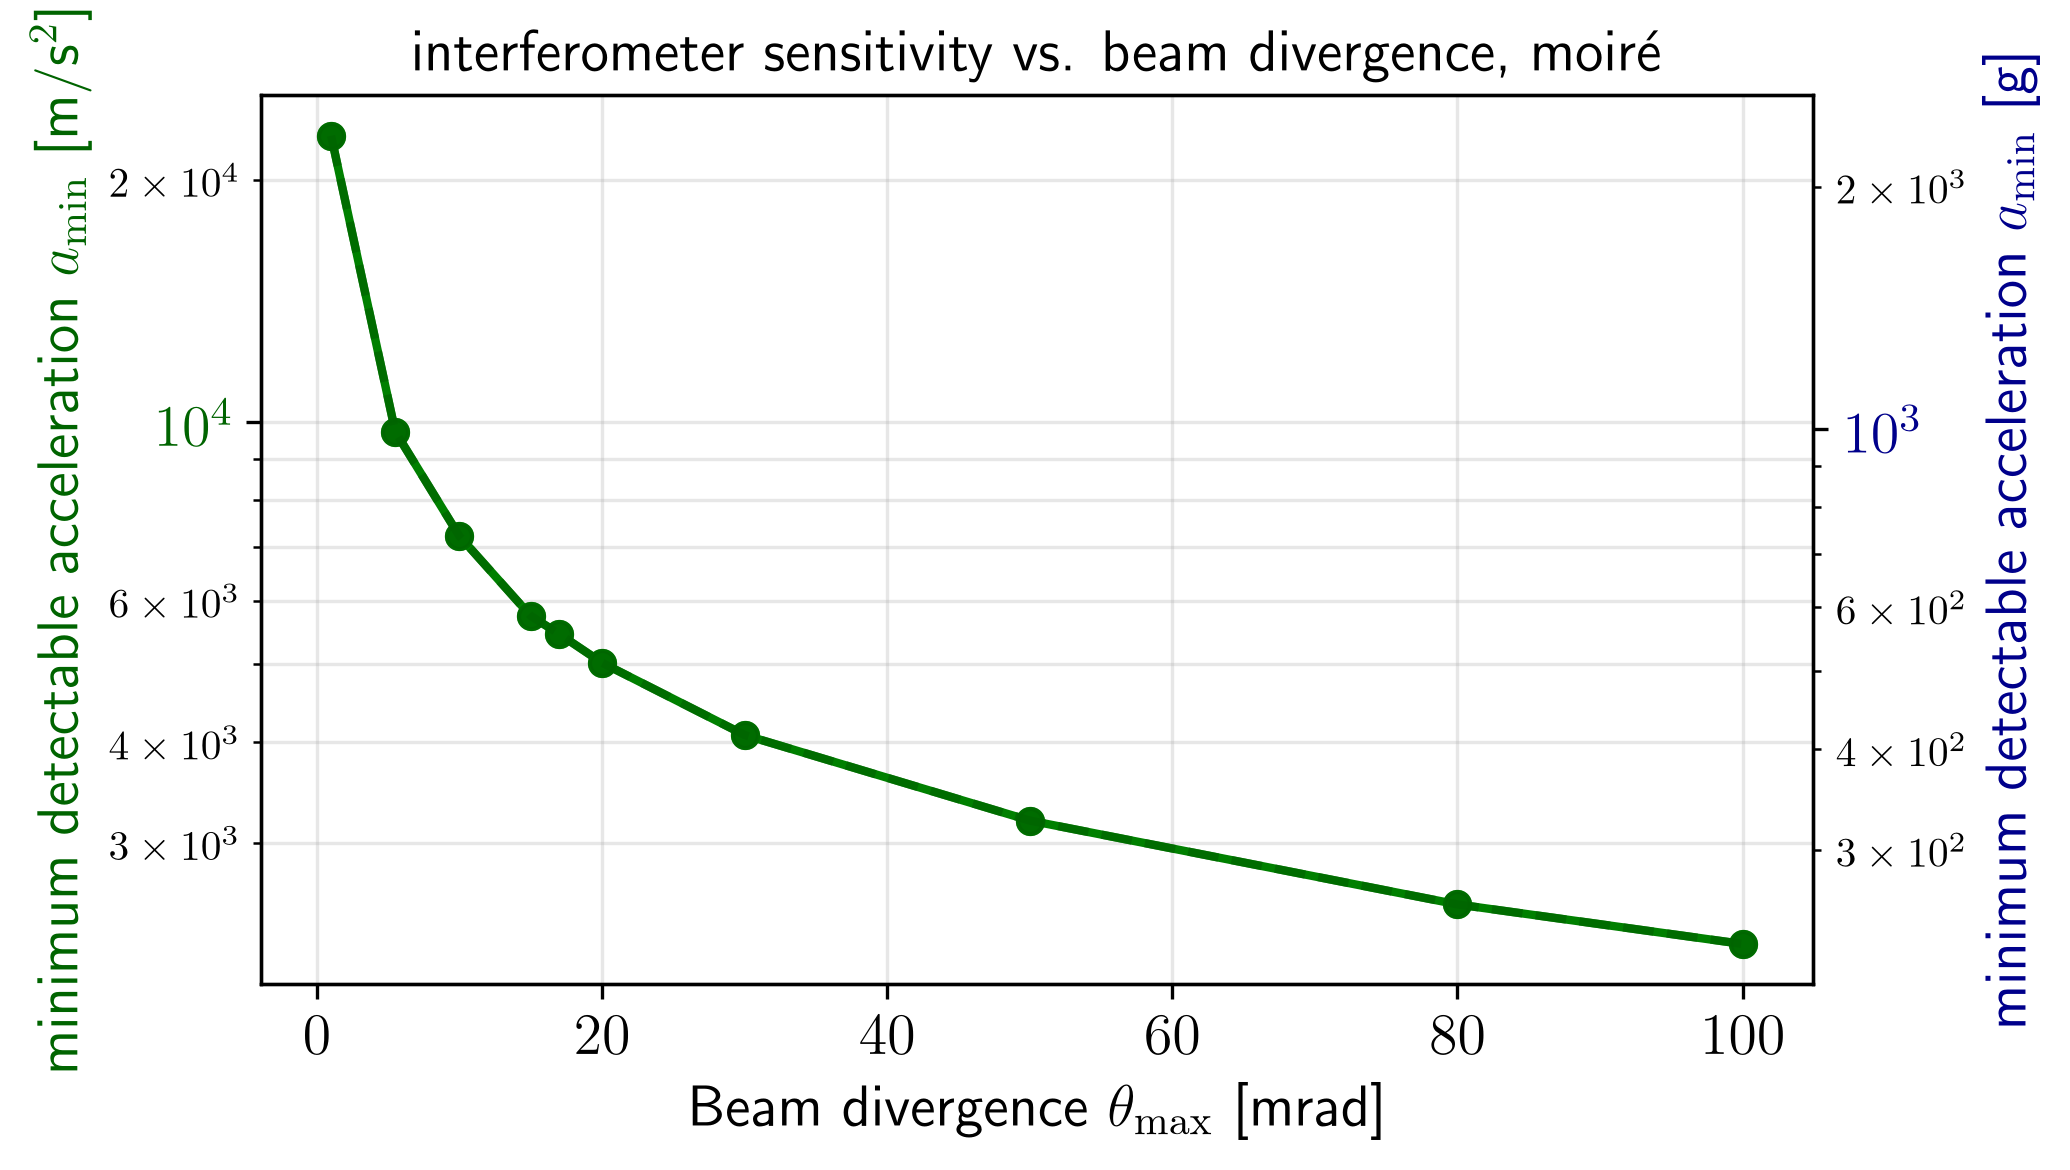
\includegraphics[width=\linewidth]{moire/moire-sens.png}
  \caption{Representative moir\'e simulation output (top) and minimum detectable acceleration as a function of beam divergence (bottom).}
  \label{fig:moire-results}
\end{figure}

\subsection{Mach--Zehnder interferometer}

In the Mach--Zehnder configuration, increasing the angular divergence eventually suppresses the interference contrast. The simulation therefore predicts an optimum divergence near $1.6\,\mathrm{mrad}$. For $8\cdot10^4$ shots, this condition corresponds to a minimum detectable acceleration of $a_{\min} = (140 \pm 1)\,\mathrm{m\,s^{-2}}$ (approximately $14.3\,g_\oplus$). Furthermore, parameter space heatmaps reveal that the optimal region on the velocity-divergence plane is very broad, meaning the setup tolerates deviations of these parameters by tens of percent without significant loss of sensitivity. The simulated phase distributions also show that gravity shifts the interference fringes in the expected direction (Fig.~\ref{fig:mz-results}).

\begin{figure}[ht!]
  \centering
  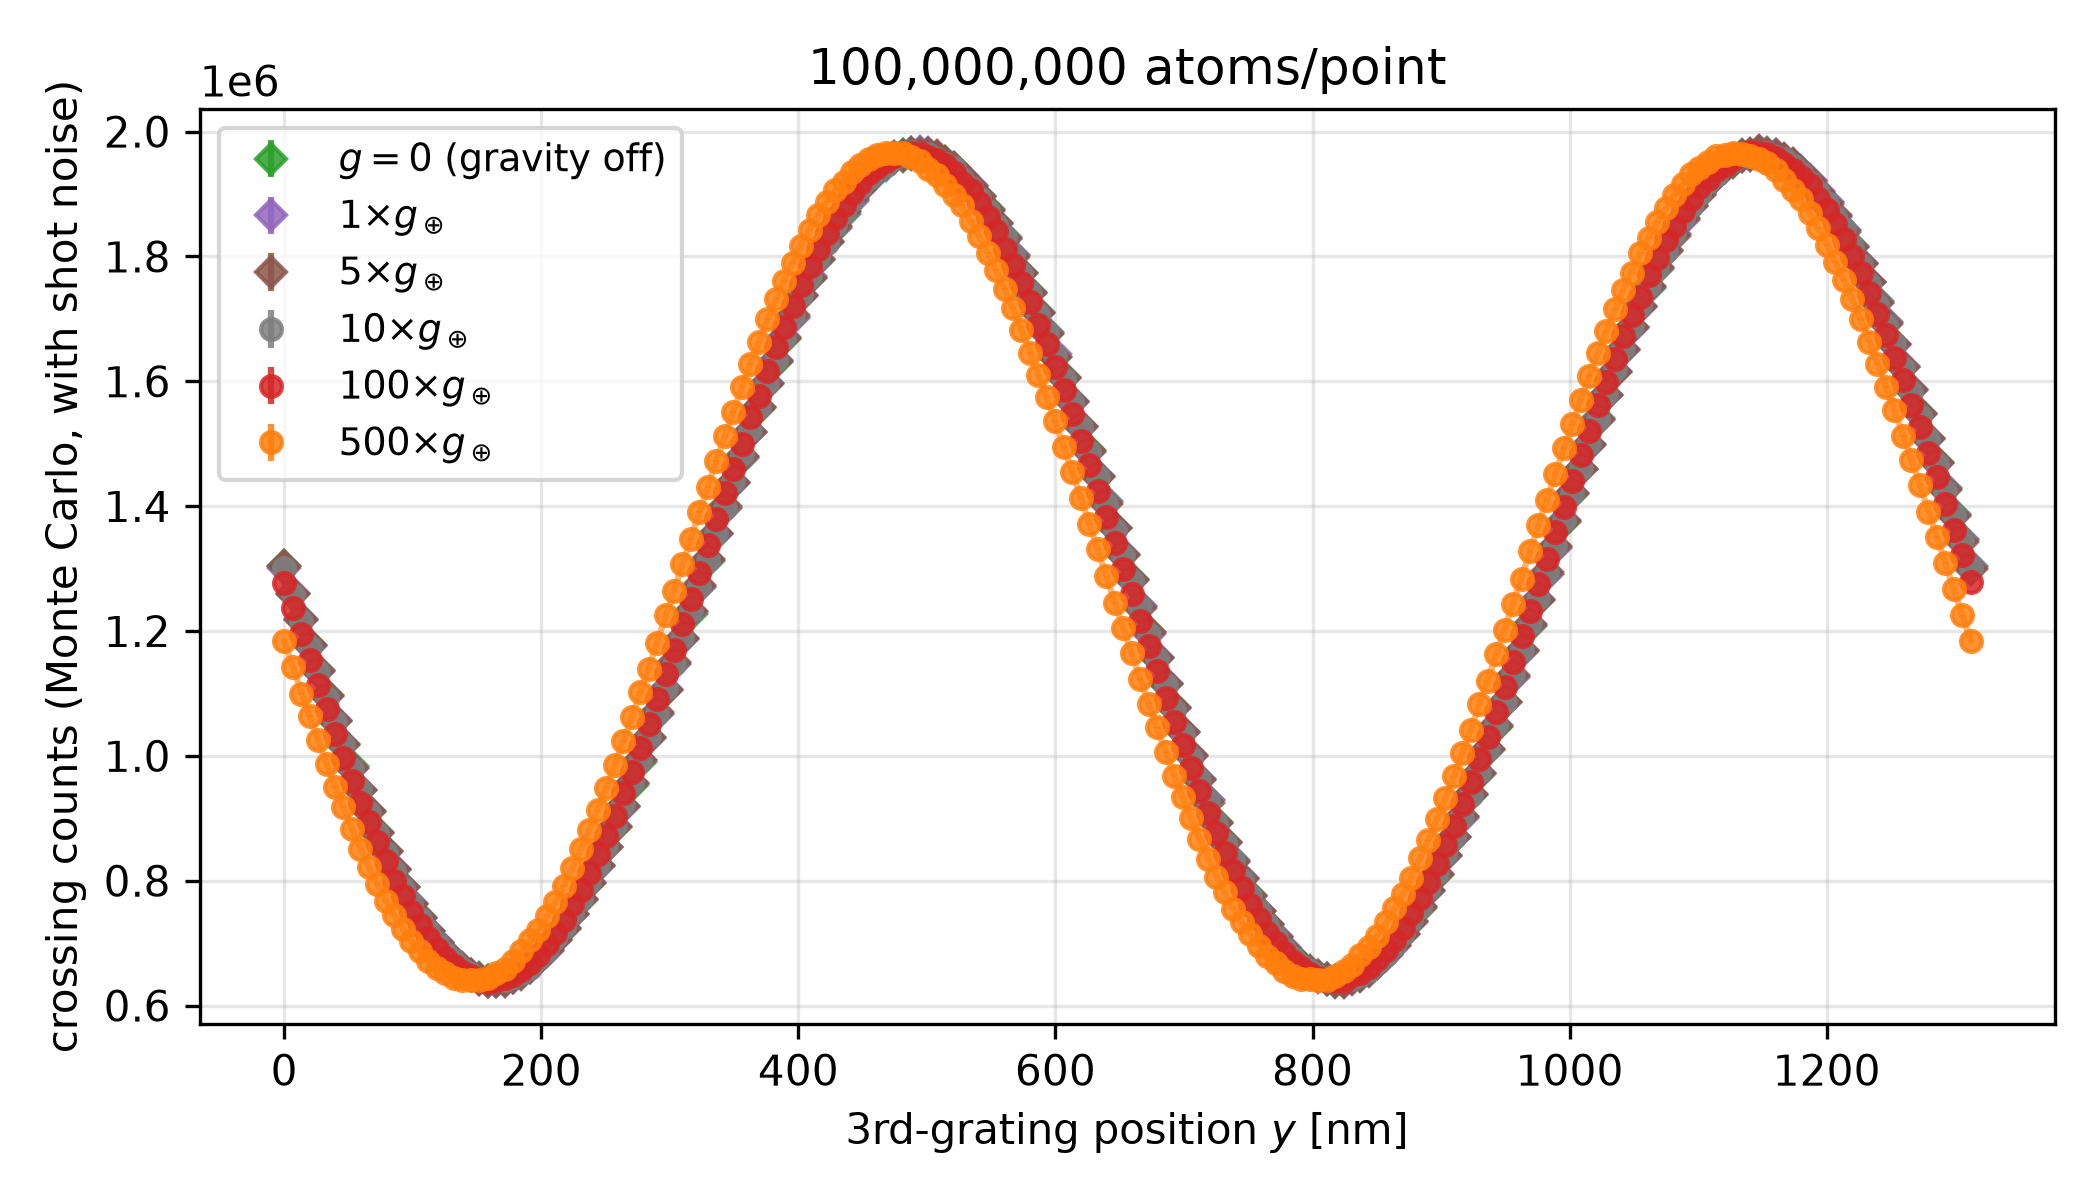
\includegraphics[width=\linewidth]{mach/mariazzi_gravity_shift_mp.png}\par\medskip
  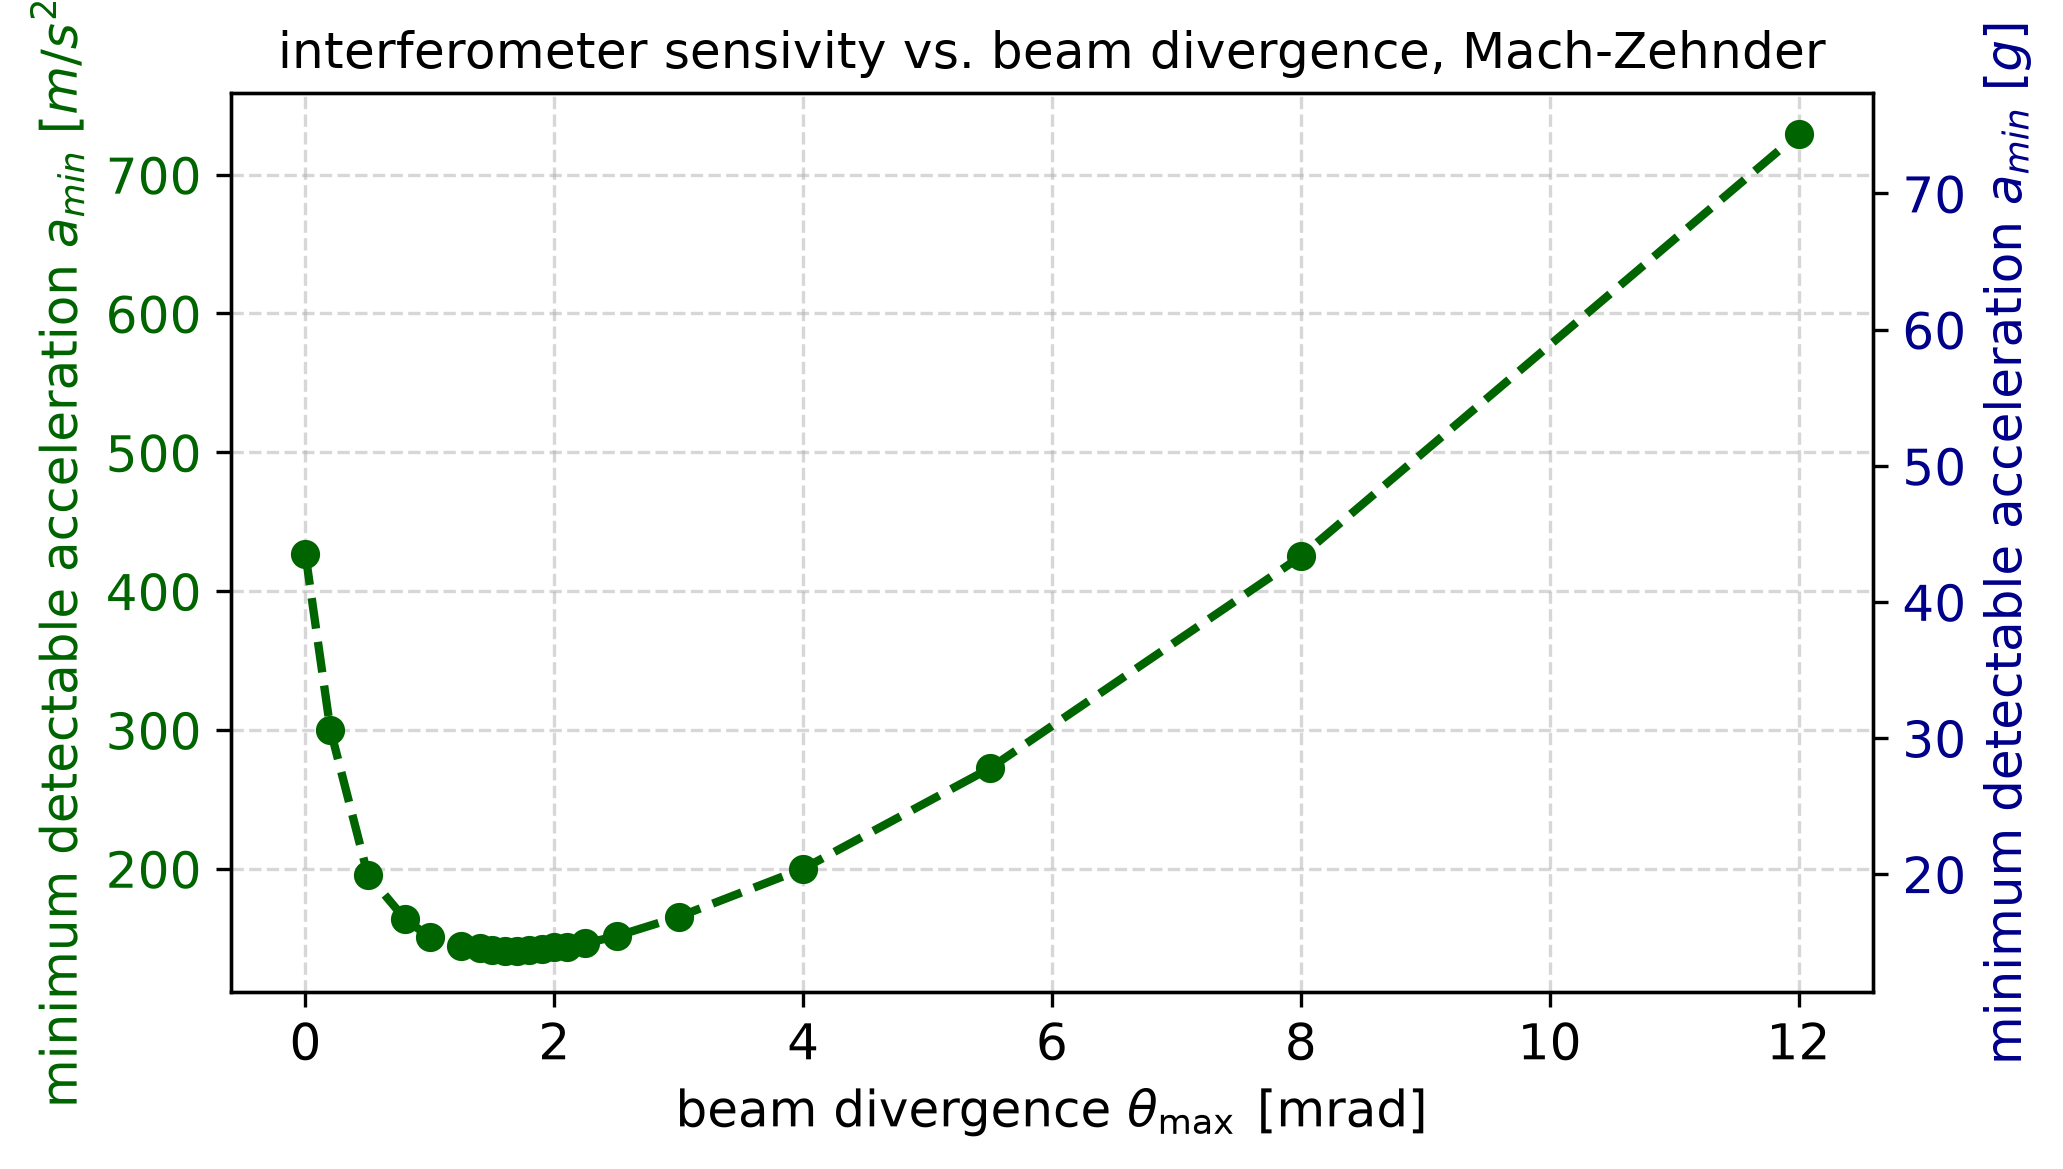
\includegraphics[width=\linewidth]{mach/mz_sensitivity_vs_divergence_dual_axis.png}
  \caption{Acceleration-induced fringe shift (top) and Mach--Zehnder sensitivity as a function of beam divergence (bottom).}
  \label{fig:mz-results}
\end{figure}

\begin{table*}[t]
    \centering
    \caption[Sensitivity comparison: simulations and literature]{Comparison of the minimum detectable accelerations \(a_{\min}\) obtained in the simulations and reported in the literature for a mean initial velocity of \(v_0=10^5\)~\si{\metre\per\second}. The simulations use 400 shots per scan point, while the literature estimates correspond to approximately 400 shots (Table 2 in \cite{Mariazzi_Caravita_Doser_Nebbia_Brusa_2020}). The beam divergences used in each case are listed in the table. Here, \(g=9.81\)~\si{\metre\per\second\squared}.}
    \label{tab:method-comparison}
    \small
    \setlength{\tabcolsep}{4pt}
    \renewcommand{\arraystretch}{1.15}
    \begin{tabular*}{\linewidth}{@{\extracolsep{\fill}}lccc@{}}
        \toprule
        Source & \(\theta_{\max}\) [mrad] & \(a_{\min}\) [\si{\metre\per\second\squared}] & \(a_{\min}/g\) \\
        \midrule
        \multicolumn{4}{@{}l}{\textbf{moir\'e}} \\
        Simulation & \(17\) & \(3408\pm31\) & \(347.4\pm3.2\) \\
        Literature & \(17\) & \(\sim 4.25\cdot10^3\) & \(\sim 4.3\cdot10^2\) \\
        \addlinespace
        \multicolumn{4}{@{}l}{\textbf{Mach--Zehnder}} \\
        Simulation & \(1.6\) & \(140\pm1\) & \(14.27\pm0.10\) \\
        Literature & \(5.5\) & \(\sim 6.9\cdot10^1\) & \(\sim 7.1\) \\
        \bottomrule
    \end{tabular*}
\end{table*}

\section{Discussion}

The calculations and simulations indicate that the Mach--Zehnder interferometer can probe substantially smaller accelerations than the moir\'e deflectometer under comparable assumptions. The main advantage is the much smaller grating period available from standing light waves. The smaller period makes a given acceleration-induced displacement a larger fraction of a fringe, improving the statistical sensitivity for short-lived particles, while the high transparency of the light gratings avoids annihilation losses on grating material.

The moir\'e deflectometer nevertheless remains attractive as a purely classical device. It does not require matter-wave coherence, and its operation can be studied directly using particle-transport simulations. It may therefore provide a useful intermediate step for validating beam formation, grating transmission, decay detection, and systematic effects.

To compare the simulations with the analytical estimates of Mariazzi et al.\ (2020)\cite{Mariazzi_Caravita_Doser_Nebbia_Brusa_2020}, the literature values are rescaled to the same total number of shots as in the simulations, i.e.\ $8\cdot10^4$, corresponding to 400 shots per scan point and 200 scan points. After this rescaling, the present Monte Carlo study demonstrates agreement within $25\%$ for the moir\'e deflectometer configuration. For the Mach--Zehnder interferometer, however, the simulation predicts a sensitivity approximately a factor of two worse than the rescaled analytical estimate. This discrepancy arises from a different modeling of the angular acceptance: replacing the sharp cut-off at the Bragg angle with a Gaussian distribution leads to a lower interference contrast.

These values should be verified with a more complete treatment of detector efficiency, background, alignment errors, velocity-dependent excitation efficiency, grating imperfections, and other experimental systematics. The dominant contributions are expected to come from grating alignment and rotation, the finite grating--stopper distance, and pick-off annihilation on the material elements.

\section{Conclusion}

Monte Carlo simulations were used to compare classical and quantum interferometric concepts for measuring gravitational effects on metastable positronium. Under the investigated assumptions, the Mach--Zehnder interferometer provides the better sensitivity, reaching approximately $14.3\,g_\oplus$ for $8\cdot10^4$ shots, compared with approximately $347.4\,g_\oplus$ for the moir\'e deflectometer. The improvement is driven mainly by the smaller grating period achievable with optical standing waves. The interferometer is therefore about 24 times more sensitive than the deflectometer, which corresponds to a 593-fold shorter measurement time for the same target acceleration. Future work will extend the simulations to include realistic detector response and systematic uncertainties and will optimize the geometry and beam parameters for an experimental implementation.

\section*{Acknowledgements}

We acknowledge support from the National Science Centre (NCN), grant nos. 2021/42/A/ST2/00423, 2021/43/B/ST2/02150, 2022/47/I/NZ7/03112, and 2023/50/E/ST2/00574; the Polish Ministry of Science and Higher Education (MNiSW), grant nos. IAL/SP/596235/2023 and SPUB/SP/627733/2025; the SciMat and qLife Priority Research Areas; and the ERC Advanced Grant POSITRONIUM (no. 101199807).

% \clearpage
\balance
\printbibliography

\end{document}